\section{Analysis of the shunted piezoelectric patches}
\label{sec:analysis_shunted_piezo}

In Section \ref{subsec:piezoelectric_patches_analysis} we have introduced the concept of shunted piezoelectric patches and we have shown how the mechanical admittance of the piezoelectric patch is influenced by the electrical impedance of the shunt circuit.

In this section, we want to further characterize this relationship by analyzing the effects of different shunt circuits on the system.
A sensitivity analysis is performed by considering the connection of the piezoelectric patches to a host beam structure and by analyzing the position of the band-gaps in the dispersion relation of the system.
While different shunting layouts are presented in the paragraph below, for the sensitivity analysis we focus on the RLC circuit only, as it is the one that is also used in the experimental analysis.

Successively, for the case of shunt circuits composed by active elements, we proposed a breif stability analysis.


\paragraph{Shunt circuits layouts}

As for the shunt circuits, three different layouts can be considered, as shown in Figure \ref{fig:shunt_layouts}.

\begin{figure}[H]

    \begin{minipage}{0.27\textwidth}

        \centering

        \begin{tikzpicture}[european voltages]

            % Upper and lower horizontal lines
            \draw (0,0) to [short] ++(3,0);
            \draw (0,-4.5) to [short] ++(3,0);

            % Piezo
            \draw (0,0) to [C, l=$C_p$, o-o] ++(0,-4.5);

            % Shunt
            \draw (3,0)
            to [R, l=$R$, o-] ++(0,-2)
            to [L, l=$L$] ++(0,-1)
            to [C, l=$C$, -o] ++(0,-1.5);

        \end{tikzpicture}

    \end{minipage}
    %
    \hfill
    %
    \begin{minipage}{0.31\textwidth}

        \centering

        \begin{tikzpicture}[european voltages]

            % Upper and lower horizontal lines
            \draw (0,0) to [short] ++(4,0);
            \draw (0,-4.5) to [short] ++(4,0);

            % Piezo
            \draw (0,0) to [C, l=$C_p$, o-o] ++(0,-4.5);

            % Shunt capacitor
            \draw (2.5,0) to [C, l=$C$, o-o] ++(0,-4.5);

            % Shunt resistor and inductor
            \draw (4,0) to [R, l=$R$, o-] ++(0,-2.5) to [L, l=$L$, -o] ++(0,-2);

        \end{tikzpicture}

    \end{minipage}
    %
    \hfill
    %
    \begin{minipage}{0.31\textwidth}

        \centering

        \begin{tikzpicture}[european voltages]

            % Upper and lower horizontal lines
            \draw (0,0) to [short] ++(4,0);
            \draw (0,-4.5) to [short] ++(4,0);

            % Piezo
            \draw (0,0) to [C, l=$C_p$, o-o] ++(0,-4.5);

            % Shunt capacitor
            \draw (2.5,0) to [R, l=$R$, o-] ++(0,-2.5) to [C, l=$C$, -o] ++(0,-2);

            % Shunt resistor and inductor
            \draw (4,0) to [L, l=$L$, o-o] ++(0,-4.5);

        \end{tikzpicture}

    \end{minipage}

    \caption{Shunt layouts: (a) Series $RLC$ shunt, (b) Parallel $RL//C$ shunt, (c) Parallel $RC//L$ shunt.}
    \label{fig:shunt_layouts}

\end{figure}

From basic circuit theory, we can write the electrical impedance of the three shunt circuits as follows:

\begin{equation}
    \begin{aligned}
        Z_{su}^{RLC}   & = R + sL + \frac{1}{sC}                                                                                          \\
        Z_{su}^{RL//C} & = \left(\frac{1}{R + sL} + sC\right)^{-1} = \frac{R + sL}{1 + (R + sL)sC} = \frac{R + sL}{1 - \omega^2LC - sRC}  \\
        Z_{su}^{RC//L} & = \left(\frac{1}{R + \frac{1}{sC}} + \frac{1}{sL} \right)^{-1} = \frac{-\omega^2 RLC + sL}{1 - \omega^2LC - sRC}
    \end{aligned}
    \label{eq:shunt_circuits_impedance}
\end{equation}

Where $s = j\omega$ is the complex frequency and $\omega$ is the angular frequency.



\paragraph{Negative capacitance realization}

When thinking to classical electrical components it's obvious, from an energetic point of view, that the values of $R$, $L$, and $C$ must be all non-negative.
However, thanks to the use of appropriate external circuits, it is possible to realize equivalent electrical components having negative values.
In particular, given that this is also the case in the experimental approach, we consider the possibility of having negative capacitance in the shunt circuits.

In order to realize a negative capacitance, the circuit depicted in Figure \ref{fig:negative_capacitance_realization} can be used.

\begin{figure}[H]
    \centering
    \begin{tikzpicture}[european voltages]

        \node[op amp] (OPAMP) {};

        \draw(OPAMP.out) to [short] ++(0, +2.9) to [C, l=$C_0$] ++(-2.5, 0) |- (OPAMP.-);
        \draw(OPAMP.out) to [short] ++(0, +1.5) to [R, l=$R_0$] ++(-2.5, 0) |- (OPAMP.-);
        \draw(OPAMP.out) to [short] ++(0, -1.5) to [R, l=$R_2$] ++(-2.5, 0) |- (OPAMP.+);

        \draw(OPAMP.-) to [short] ++(-2, 0);
        \draw(OPAMP.+) to [R, l=$R_1$] ++(-2, 0);

    \end{tikzpicture}
    \caption{Negative capacitance realization using an OP-AMP.}
    \label{fig:negative_capacitance_realization}

\end{figure}

The circuit depicted in Figure \ref{fig:negative_capacitance_realization} is equivalent to a negative capacitance having the following value:

\begin{equation}
    C_{eq} = -C_N = -\frac{R_1}{R_2} \left(\frac{1}{R_0} + sC_0\right)^{-1}
    \label{eq:negative_capacitance_real}
\end{equation}

One can notice the presence of the resistance $R_0$ parallel to the capacitance $C_0$.
While $R_1$ and $R_2$ are used to scale the value of the negative capacitance, $R_0$ is a key component of the circuit that enable a bias path for the current flowing through the negative capacitance avoiding the saturation of the OP-AMP.
Ideally, $R_0$ should be infinite, leading to the following expression for the ideal negative capacitance:

\begin{equation}
    C_{eq} = -C_N = -\frac{R_1}{R_2} \left(sC_0\right)^{-1}
    \label{eq:negative_capacitance_ideal}
\end{equation}

Of course, being the OP-AMP an active element powered by an external power supply, its presence in the circuit can lead to instability issues.
A dedicated analysis focusing on this aspect is proposed in Section \ref{subsec:stability_analysis}.


\subsection{Sensitivity analysis}
\label{subsec:sensitivity_analysis}

For the study of the system's band-gaps, we consider the connection of the piezoelectric patches to a beam structure as shown in Figure \ref{fig:beam_piezo_patches}.
The same numerical values for the geometry and material properties used in the experimental setup are considered (see Section \ref{subsec:experimental_setup}).

\begin{figure}[H]

    \centering

    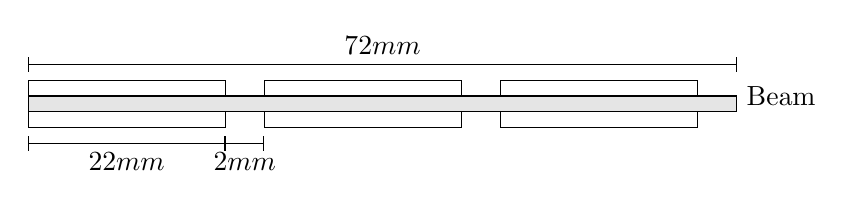
\begin{tikzpicture}

        % Beam
        \draw[fill=gray!20] (0,0) rectangle (9,0.2) node[right] {Beam};

        \draw[|-|] (0,0.6) -- (9,0.6) node[pos=.5, above] {$72 mm$};
        \draw[|-|] (0,-0.4) -- (2.5,-0.4) node[pos=.5, below] {$22 mm$};
        \draw[|-|] (2.5,-0.4) -- (3,-0.4) node[pos=.5, below] {$2 mm$};


        \foreach  \i in {0,1,2}
            {
                % Piezo patches
                \draw[fill=white] (3*\i, 0.2) rectangle (2.5 + 3*\i, 0.4);
                \draw[fill=white] (3*\i, 0.0) rectangle (2.5 + 3*\i, -0.2);
            }

    \end{tikzpicture}

    \caption{Unit cell composed by a beam substrate and 3 pairs of piezoelectric patches.}
    \label{fig:beam_piezo_patches}

\end{figure}

Intuitively, the presence of the piezoelectric patches will cause a change in the mechanical properties of the beam.
For simplicity, a weighted average of the mechanical properties of the beam and the piezoelectric patches is considered:

\begin{equation}
    \begin{aligned}
        J^*    & = J_b + 2 J_p                                   \\
        A^*    & = A_b + 2 A_p                                   \\
        E^*    & = \frac{E_b J_b + 2 E_p J_p}{J_b + 2 J_p}       \\
        \rho^* & = \frac{\rho_b A_b + 2 \rho_p A_p}{A_b + 2 A_p}
    \end{aligned}
    \label{eq:weighted_average_mechanical_properties}
\end{equation}


\subsubsection{$RLC_N$ shunt circuit}
\label{subsubsec:RLC_shunt_circuit_negative_capacitance}

The electrical impedance of an $RLC_N$ shunt circuit is given by Equation \ref{eq:shunt_circuits_impedance}, in which $C$ takes the form of $-C_N$.
By substitution in Equation \ref{eq:mechanical_admittance_shunted_piezoelectric_patch}, we obtain the mechanical admittance of the piezoelectric patch connected to the $RLC_N$ shunt circuit as:

\begin{equation}
    Y^{SU} = Y_1^D \left( 1 - \frac{k_{31}^2}{1 + s C_p^S \left( R + sL - \frac{1}{sC_N} \right)} \right) = Y_1^D \left( 1 - \frac{k_{31}^2}{1 + C_p^S \left( -\frac{1}{C_N} - \omega^2 L \right) - s C_p^S R} \right)
    \label{eq:mechanical_admittance_RLC_shunt}
\end{equation}

It's intuitive to think that the presence of the shunt circuit will cause a variation in the piezoelectric coupling coefficient.
This means that via a proper choice of the shunt circuit parameters, it's possible to control the mechanical admittance of the piezoelectric patch and, consequently, the band-gap of the system.
In particular, the new coupling coefficient can be written as:

\begin{equation}
    (k_{31}^{SU})^2 = \frac{k_{31}^2}{1 + C_p^S \left( -\frac{1}{C_N} - \omega^2 L \right) - s C_p^S R}
    \label{eq:coupling_coefficient_RLC_shunt}
\end{equation}

By analyzing the above equation, it's possible to understand that $R$ act as damping factor being multiplied by the complex frequency $s$.
This means that $R$ can be used to control the width and the depth of the band-gap.
On the other hand, $L$ and $C_N$ can be used to shift the band-gap to lower or higher frequencies, given that their contribution decreases or increases the stiffness of the undergoing structure.

The following figures, shows the dispersion relation of the system for different values of $R$, $L$, and $C$.
All the plots are obtained by using the Transfer Matrix Method (TMM).


\paragraph{Short circuit case}

In the short circuit case, the impedance of the shunt circuit is given by $Z_{su} = 0 \Omega$.
In this case, the mechanical admittance of the piezoelectric patch is actually the same as the one of the piezoelectric patch itself $Y^{SU} = Y_1^E$ in the null electric field case.

\begin{figure}[H]
    \centering
    \includegraphics[width=\textwidth]{./img/MATLAB/TMM_ON-ON-ON_OFF_R1000_L0.015_C5e-09.pdf}
    \caption{Short circuit case.}
    \label{fig:TMM_ON-ON-ON_OFF_R1000_L0.015_C5e-09.pdf}
\end{figure}


\paragraph{Open circuit case}

In the open circuit case, the impedance of the shunt circuit is given by $Z_{su} = \infty \Omega$.
In this case, for the mechanical admittance of the piezoelectric patch, we have $Y^{SU} = Y_1^D$.
The dispersion relation of the system is shown in Figure \ref{fig:TMM_ON-ON-ON_+inf_R1000_L0.015_C5e-09.pdf}.

\begin{figure}[H]
    \centering
    \includegraphics[width=\textwidth]{./img/MATLAB/TMM_ON-ON-ON_+inf_R1000_L0.015_C5e-09.pdf}
    \caption{Open circuit case.}
    \label{fig:TMM_ON-ON-ON_+inf_R1000_L0.015_C5e-09.pdf}
\end{figure}

With respect to the short circuit case, the band-gap is shifted to higher frequencies due to the fact that the structure is now stiffer ($Y_1^D > Y_1^E$).


\paragraph{$L$ shunt circuit}

In the case of a purely inductive shunt circuit, the impedance is given by $Z_{su} = sL$, and the equation for the mechanical admittance of the piezoelectric patch reduces to:

\begin{equation}
    Y^{SU} = Y_1^D \left( 1 - \frac{k_{31}^2}{1 -\omega^2 C_p^S L} \right)
    \label{eq:mechanical_admittance_R_shunt}
\end{equation}

For the analysis, four values of $L$ are considered while $R$ and $C_N$ are kept constant at $0 \Omega$ and $\infty F$, respectively.

\begin{table}[H]
    \centering
    \begin{tabular}{|c|c|c|}
        \hline
        $R$ [$\Omega$] & $L$ [H] & $C_N$ [F] \\
        \hline
        0              & 0.00    & $\infty$  \\
        0              & 0.02    & $\infty$  \\
        0              & 0.10    & $\infty$  \\
        0              & 1.00    & $\infty$  \\
        \hline
    \end{tabular}
    \caption{Values of $R$, $L$, and $C_N$ for the purely inductive shunt circuit.}
    \label{tab:RLC_N_values_L_case}
\end{table}

One can also visualize the effect of the inductive element on the system by plotting $Y^{SU}$ for the different values of $L$.

\begin{figure}[H]
    \centering
    \includegraphics[width=0.6\textwidth]{./img/MATLAB/Y_SU_Purely inductive shunt circuit.pdf}
    \caption{Analysis of $Y^{SU}$ for the purely inductive shunt circuit.}
    \label{fig:Y_SU_Purely_inductive_shunt_circuit.pdf}
\end{figure}

Instead, the dispersion relation of the system are shown in the figures below.

\begin{figure}[H]
    \centering
    \includegraphics[width=\textwidth]{./img/MATLAB/TMM_ON-ON-ON_RLC_R0_L0_CInf.pdf}
    \caption{RLC shunt circuit with $R = 0 \Omega$, $L = 0 H$, and $C = \infty F$.}
    \label{fig:TMM_ON-ON-ON_RLC_R0_L0_CInf.pdf}
\end{figure}

\begin{figure}[H]
    \centering
    \includegraphics[width=\textwidth]{./img/MATLAB/TMM_ON-ON-ON_RLC_R0_L0.02_CInf.pdf}
    \caption{RLC shunt circuit with $R = 0 \Omega$, $L = 0.02 H$, and $C = \infty F$.}
    \label{fig:TMM_ON-ON-ON_RLC_R0_L0.02_CInf.pdf}
\end{figure}

\begin{figure}[H]
    \centering
    \includegraphics[width=\textwidth]{./img/MATLAB/TMM_ON-ON-ON_RLC_R0_L0.1_CInf.pdf}
    \caption{RLC shunt circuit with $R = 0 \Omega$, $L = 0.10 H$, and $C = \infty F$.}
    \label{fig:TMM_ON-ON-ON_RLC_R0_L0.1_CInf.pdf}
\end{figure}

\begin{figure}[H]
    \centering
    \includegraphics[width=\textwidth]{./img/MATLAB/TMM_ON-ON-ON_RLC_R0_L1_CInf.pdf}
    \caption{RLC shunt circuit with $R = 0 \Omega$, $L = 1 H$, and $C = \infty F$.}
    \label{fig:TMM_ON-ON-ON_RLC_R0_L1_CInf.pdf}
\end{figure}

Based also on Figure \ref{fig:Y_SU_Purely_inductive_shunt_circuit.pdf}, it's possible to observe that at low frequencies the system behaves as in the short circuit case, while at higher frequencies the system behaves as in the open circuit case.
Moreover, the lower $L$, the higher the frequency at which the transition between the two behaviors occurs.
The transition frequency between the two behaviors is given by:

\begin{equation}
    1 - \omega^2 C_p^S L = 0 \rightarrow \omega_n = \frac{1}{\sqrt{C_p^S L}}
\end{equation}

When the natural frequency falls within the band-gap, a splitting of the band-gap occurs, as shown in Figure \ref{fig:TMM_ON-ON-ON_RLC_R0_L0.1_CInf.pdf}.
One might use this effect to create an isolated band-pass filter.


\paragraph{$RL$ shunt circuit}

In the case of a resistive-inductive shunt circuit, the impedance is given by $Z_{su} = R + sL$.
The equation for the mechanical admittance of the piezoelectric patch is:

\begin{equation}
    Y^{SU} = Y_1^D \left( 1 - \frac{k_{31}^2}{1 -\omega^2 C_p^S L - s C_p^S R} \right)
    \label{eq:mechanical_admittance_RL_shunt}
\end{equation}

For the analysis, four values of $R$ are considered while $L$ and $C_N$ are kept constant at $0.03 H$ and $\infty F$, respectively.

\begin{table}[H]
    \centering
    \begin{tabular}{|c|c|c|}
        \hline
        $R$ [$\Omega$] & $L$ [H] & $C_N$ [F] \\
        \hline
        0              & 0.03    & $\infty$  \\
        50             & 0.03    & $\infty$  \\
        200            & 0.03    & $\infty$  \\
        1000           & 0.03    & $\infty$  \\
        \hline
    \end{tabular}
    \caption{Values of $R$, $L$, and $C_N$ for the resistive-inductive shunt circuit.}
    \label{tab:RLC_N_values_RL_case}
\end{table}

One can also visualize the effect of the resistive element on the system by plotting $Y^{SU}$ for the different values of $R$.

\begin{figure}[H]
    \centering
    \includegraphics[width=0.6\textwidth]{./img/MATLAB/Y_SU_Resistive-Inductive shunt circuit.pdf}
    \caption{Analysis of $Y^{SU}$ for the resistive-inductive shunt circuit.}
    \label{fig:Y_SU_Resistive-Inductive_shunt_circuit.pdf}
\end{figure}

Instead, the dispersion relation of the system are shown in the figures below.

\begin{figure}[H]
    \centering
    \includegraphics[width=\textwidth]{./img/MATLAB/TMM_ON-ON-ON_RLC_R0_L0.03_CInf.pdf}
    \caption{RLC shunt circuit with $R = 0 \Omega$, $L = 0.03 H$, and $C = \infty F$.}
    \label{fig:TMM_ON-ON-ON_RLC_R0_L0.03_CInf.pdf}
\end{figure}

\begin{figure}[H]
    \centering
    \includegraphics[width=\textwidth]{./img/MATLAB/TMM_ON-ON-ON_RLC_R50_L0.03_CInf.pdf}
    \caption{RLC shunt circuit with $R = 50 \Omega$, $L = 0.03 H$, and $C = \infty F$.}
    \label{fig:TMM_ON-ON-ON_RLC_R50_L0.03_CInf.pdf}
\end{figure}

\begin{figure}[H]
    \centering
    \includegraphics[width=\textwidth]{./img/MATLAB/TMM_ON-ON-ON_RLC_R200_L0.03_CInf.pdf}
    \caption{RLC shunt circuit with $R = 200 \Omega$, $L = 0.03 H$, and $C = \infty F$.}
    \label{fig:TMM_ON-ON-ON_RLC_R200_L0.03_CInf.pdf}
\end{figure}

\begin{figure}[H]
    \centering
    \includegraphics[width=\textwidth]{./img/MATLAB/TMM_ON-ON-ON_RLC_R1000_L0.03_CInf.pdf}
    \caption{RLC shunt circuit with $R = 1000 \Omega$, $L = 0.03 H$, and $C = \infty F$.}
    \label{fig:TMM_ON-ON-ON_RLC_R1000_L0.03_CInf.pdf}
\end{figure}

Based also on Figure \ref{fig:Y_SU_Resistive-Inductive_shunt_circuit.pdf}, it's possible to observe that at low frequencies the system behaves as in the short circuit case, while at higher frequencies the system behaves as in the open circuit case, similarly to the purely inductive case.

However, the main difference is that the resistive element $R$ acts as a damping factor, which can be used to control the width and the depth of the band-gap.
This phenomenon is clearly visible in the dispersion relation plots, where the central position of the band-gap remains the same (governed by $L$ only), while the attenuation level decreases with increasing $R$.
For high values of $R$, regardless of the value of $L$, the band-gap can be completely suppressed.



\paragraph{$RC_N$ shunt circuit}

In the case of a resistive-(negative) capacitive shunt circuit, the impedance of the shunt circuit is given by $Z_{su} = R - \frac{1}{sC_N}$.
The equation for the mechanical admittance of the piezoelectric patch is:

\begin{equation}
    Y^{SU} = Y_1^D \left( 1 - \frac{k_{31}^2}{1 - C_p^S \frac{1}{C_N} - s C_p^S R} \right)
    \label{eq:mechanical_admittance_RC_shunt}
\end{equation}

For the analysis, three values of $C_N$ are considered while $R$ and $L$ are kept constant at $1000 \Omega$ and $0H$, respectively.

\begin{table}[H]
    \centering
    \begin{tabular}{|c|c|c|}
        \hline
        $R$ [$\Omega$] & $L$ [H] & $C_N$ [F] \\
        \hline
        1000           & 0       & 30e-9     \\
        1000           & 0       & 7e-9      \\
        1000           & 0       & 5e-9      \\
        \hline
    \end{tabular}
    \caption{Values of $R$, $L$, and $C_N$ for the resistive-(negative) capacitive shunt circuit.}
    \label{tab:RLC_N_values_RC_case}
\end{table}

One can also visualize the effect of the capacitive element on the system by plotting $Y^{SU}$ for the different values of $C_N$.

\begin{figure}[H]
    \centering
    \includegraphics[width=0.6\textwidth]{./img/MATLAB/Y_SU_Resistive-(Negative) Capacitive shunt circuit.pdf}
    \caption{Analysis of $Y^{SU}$ for the resistive-(negative) capacitive shunt circuit.}
    \label{fig:Y_SU_Resistive-(Negative)_Capacitive_shunt_circuit.pdf}
\end{figure}

Instead, the dispersion relation of the system are shown in the figures below.

\begin{figure}[H]
    \centering
    \includegraphics[width=\textwidth]{./img/MATLAB/TMM_ON-ON-ON_RLC_R1000_L0_C-3e-08.pdf}
    \caption{RLC shunt circuit with $R = 1000 \Omega$, $L = 0 H$, and $C = -30 nF$.}
    \label{fig:TMM_ON-ON-ON_RLC_R1000_L0_C-30e-09.pdf}
\end{figure}

\begin{figure}[H]
    \centering
    \includegraphics[width=\textwidth]{./img/MATLAB/TMM_ON-ON-ON_RLC_R1000_L0_C-7e-09.pdf}
    \caption{RLC shunt circuit with $R = 1000 \Omega$, $L = 0 H$, and $C = -7 nF$.}
    \label{fig:TMM_ON-ON-ON_RLC_R1000_L0_C-7e-09.pdf}
\end{figure}

\begin{figure}[H]
    \centering
    \includegraphics[width=\textwidth]{./img/MATLAB/TMM_ON-ON-ON_RLC_R1000_L0_C-5e-09.pdf}
    \caption{RLC shunt circuit with $R = 1000 \Omega$, $L = 0 H$, and $C = -5 nF$.}
    \label{fig:TMM_ON-ON-ON_RLC_R1000_L0_C-5e-09.pdf}
\end{figure}

The effect of the negative capacitance is to shift the band-gap frequencies.
Depending on the sign of $1 - C_p^S \frac{1}{C_N}$, the band-gap can be shifted to higher (negative sign) or lower (positive sign) frequencies.
This effect can be used to tune the band-gap to a desired frequency range.

Notice however that the introduction of a negative capacitance can lead to instability issues, as the system can become underdamped.
Not all the configurations shown in the figures above are in fact stable, the purpose of this analysis is to show the effect of the negative capacitance on the system's band-gap and not to provide a stable configuration.





\subsection{Stability analysis}
\label{subsec:stability_analysis}

As introduced at the beginning this section, a shunting circuit can be either passive or active.
While passive shunts are stable by definition (conservation of energy), active shunts can introduce instabilities in the system.

In particular, considering piezoelectric patches connected to a shunting circuts, two types of instabilities can be introduced:

\begin{itemize}
    \item \textbf{Mechanical instability}: the equivalent stiffness of the piezoelectric patch become negative;
    \item \textbf{Electrical instability}: the equivalent capacitance of the electrical circuit becomes negative.
\end{itemize}

For the sake of simplicity, we consider here only the case of the purely capacitance shunting circuit, with a series connection between the piezoelectric patch and the shunt capacitor (similar to the one shown in Figure \ref{fig:shunt_layouts} (a)).


\subsubsection{$C_N$ shunting circuit}
\label{subsubsec:stability_analysis_negative_capacitance}

As already discussed, the negative capacitance shunting circuit is a particular case of active shunt circuit that can be implemented via OP-AMPs as explained at the beginning of the section.

In this case, considering $Z_{SU} = -\frac{1}{sC_N}$, the mechanical admittance of the piezoelectric patch can be written as:

\begin{equation}
    Y^{SU} = Y_1^D \left( 1 - \frac{k_{31}^2}{1 - C_p^S \frac{1}{C_N}} \right)
\end{equation}

If we consider the ideal case for the shunting circuit, we have already shown in Equation \ref{eq:negative_capacitance_ideal} that the value of $C_N$ doesn't depend on the value of $s = j\omega$.
This means that instability properties (at least in the ideal case) are not frequency-dependent, but rather depends only on the selected value of $C_N$.

In Figure \ref{fig:stability_analysis_negative_capacitance} we show the normalized mechanical admittance of the piezoelectric patch function of the normalized capacitance of the shunting circuit.

\begin{figure}[H]
    \centering
    \includegraphics[width=0.5\textwidth]{./img/MATLAB/Stability_analysis_C_N.pdf}
    \caption{Stability analysis of the negative capacitance shunting circuit.}
    \label{fig:stability_analysis_negative_capacitance}
\end{figure}

The colored regions in the plot highlight the regions of mechanical instability (blue) and electrical instability (green).
The red region instead highlights the region where $C_N$ is negative, which means having positive capacitance in the shunting circuit ($C_{eq} = -C_N$).


\paragraph{Mechanical instability}

The mechanical instability region is defined by the condition:

\begin{equation}
    Y^{SU} < 0 \rightarrow 1 - \frac{k_{31}^2}{1 - C_p^S \frac{1}{C_N}} < 0
\end{equation}


\paragraph{Electrical instability}

The electrical instability region is defined by the condition:

\begin{equation}
    C_{tot} = \left( \frac{1}{C_p^T} - \frac{1}{C_N} \right)^{-1} < 0
\end{equation}

Re-arranging the terms, we have:

\begin{equation}
    C_N < C_p^T
\end{equation}



